\documentclass{article}
\usepackage{multicol}
\usepackage{booktabs}
\usepackage{ragged2e}
\usepackage{array}
\usepackage{tikz}
\usetikzlibrary{calc}
\usepackage{amsmath}
\usepackage{amssymb}

\title{Translational Motion Concept Map}
\author{Timothy C. Burt}

\begin{document}
\maketitle
\begin{multicols}{2}

%\usepackage{tikz}
%\usetikzlibrary{calc}
%\usepackage{amsmath}


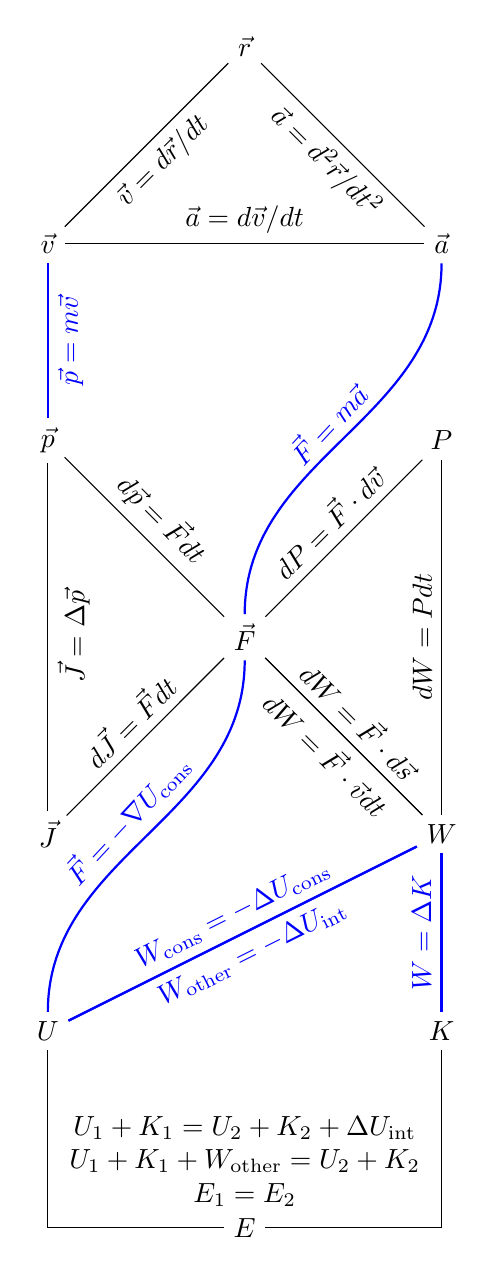
\begin{tikzpicture}
  \def\baseSep{2.5}
  % Energy section: nodes
  \node (E) at (\baseSep, 0) {$E$};
  \node (U) at ($(E)+(-\baseSep,\baseSep)$) {$U$};
  \node (K) at ($(E)+(\baseSep,\baseSep)$) {$K$};

  % Force section: nodes
  \node (vF) at ($(E)+(0, 3*\baseSep)$) {$\vec{F}$};
  \node (vJ) at ($(vF)+(-\baseSep, -\baseSep)$) {$\vec{J}$};
  \node (W) at ($(vF)+(\baseSep, -\baseSep)$) {$W$};
  \node (vp) at ($(vF)+(-\baseSep, \baseSep)$) {$\vec{p}$};
  \node (P) at ($(vF)+(\baseSep, \baseSep)$) {$P$};

  % Descriptor section: nodes
  \node (vr) at ($(vF)+(0,3*\baseSep)$) {$\vec{r}$};
  \node (vv) at ($(vr)+(-\baseSep, -\baseSep)$) {$\vec{v}$};
  \node (va) at ($(vr)+(\baseSep, -\baseSep)$) {$\vec{a}$};


  % Descriptor section: connections
  \draw (vv) -- (vr) node [midway, below, sloped] %
  {$\vec{v}=d\vec{r}/dt$};
  \draw (vr) -- (va) node [midway, below, sloped] %
  {$\vec{a}=d^2\vec{r}/dt^2$}; 
  \draw (vv) -- (va) node [midway, above, sloped] %
  {$\vec{a}=d\vec{v}/dt$}; 

  % Force section: connections
  \draw (vp) -- (vF) node [midway, above, sloped] %
  {$d\vec{p}=\vec{F}dt$};
  \draw (vF) -- (P) node [midway, above, sloped] %
  {$dP=\vec{F}\cdot d\vec{v}$};
  \draw (vF) -- (W) node [midway, above, sloped] %
  {$dW=\vec{F}\cdot d\vec{s}$};
  \draw (vF) -- (W) node [midway, below, sloped] %
  {$dW=\vec{F}\cdot \vec{v}dt$};
  \draw (vJ) -- (vF) node [midway, above, sloped] %
  {$d\vec{J}=\vec{F}dt$};
  \draw (vJ) -- (vp) node [midway, below, sloped] %
  {$\vec{J}=\Delta\vec{p}$};
  \draw (W) -- (P) node [midway, above, sloped] %
  {$dW=P dt$};

  % Energy section: connections
  \draw (U) |- (E);
  \draw (K) |- (E);
  \node (consE-abstract) at ($(E)+(0,\baselineskip)$) %
  {$E_1=E_2$};
  \node (consE-Wother) at ($(E)+(0,2*\baselineskip)$) %
  {$U_1+K_1+W_{\text{other}}=U_2+K_2$};
  \node (consE-Uint) at ($(E)+(0,3*\baselineskip)$) %
  {$U_1+K_1=U_2+K_2+\Delta U_{\text{int}}$};

  % Inter section: connections
  % Energy and force
  \draw [thick, blue] (U) -- (W) node [midway, above, sloped, blue] %
  {$W_{\text{cons}}=-\Delta U_{\text{cons}}$};
  \draw [thick, blue] (U) -- (W) node [midway, below, sloped, blue] %
  {$W_{\text{other}}=-\Delta U_{\text{int}}$};
  \draw [thick, blue] (K) -- (W) node [midway, above, sloped, blue] %
  {$W=\Delta K$};
  \draw [thick, blue] (U) to[out=90, in=-90] (vF);
  \path (U) -- (vF) node [midway, above, rotate=47, blue] % 
  {$\vec{F} = -\nabla U_{\text{cons}}$};
  % Force and descriptors
  \draw [thick, blue] (vF) to[out=90, in=-90] (va);
  \path (vF) -- (va) node [midway, above, rotate=47, blue] %
  {$\vec{F}=m\vec{a}$};
  \draw [thick, blue] (vp) -- (vv) node [midway, below, sloped, blue] %
  {$\vec{p}=m\vec{v}$};
\end{tikzpicture}


\begin{tabular}{>{$}l<{$}>{\RaggedRight}p{0.8\linewidth}}
  \toprule
  t & time \\
  \vec{r} & position\\
  \vec{v} & velocity\\
  \vec{a} & acceleration\\
  \midrule
  m & mass\\
  \vec{p} & momentum\\
  \vec{F} & force\\
  P & power\\
  \vec{J} & impulse\\
  W & work\\
  \midrule %
  U & potential energy\\
  K & kinetic energy\\
  U_{\text{cons}} & potential due to conservative interactions\\
  W_{\text{cons}} & work done by conservative interactions\\
  U_{\text{int}} & internal energy\\
  W_{\text{other}} & work done by interactions not accounted for explicitly\\
  E & total energy\\
  \midrule %
  q & generic variable for discussion of operations\\
  \Delta q & difference between final and initial values of $q$ ($\Delta q
  \equiv q_{\text{final}} - q_{\text{initial}}$)\\
  dq & differential element $q$\\
  \vec{q}_1\cdot\vec{q}_2 & scalar (dot) product between $q_1$ and $q_2$
  ($\vec{q}_1\cdot\vec{q}_2 = |\vec{q}_1||\vec{q}_2|\cos(\phi_{1,2})$)\\
  \nabla q & gradient of the scalar $q$\\
  \bottomrule
\end{tabular}
\end{multicols}
\end{document}
